\documentclass[conference]{IEEEtran}
\IEEEoverridecommandlockouts
% The preceding line is only needed to identify funding in the first footnote. If that is unneeded, please comment it out.
\usepackage{cite}
\usepackage{amsmath,amssymb,amsfonts}
\usepackage{algorithmic}
\usepackage{graphicx}
\usepackage{textcomp}
\usepackage{xcolor}
\usepackage{emoji}
\usepackage{minted}

\def\BibTeX{{\rm B\kern-.05em{\sc i\kern-.025em b}\kern-.08em
    T\kern-.1667em\lower.7ex\hbox{E}\kern-.125emX}}
\begin{document}

\title{Covert Channel Using Github Reactions \\
% {\footnotesize \textsuperscript{*}Note: Sub-titles are not captured in Xplore and
% should not be used}
% \thanks{Identify applicable funding agency here. If none, delete this.}
}

\author{
\IEEEauthorblockN{1\textsuperscript{st} Rajeev Karuvath}
\IEEEauthorblockA{
% \textit{Computing Security Department} \\
\textit{Rochester Institute of Technology}\\
% City, Country \\
rk3824@rit.edu}
\and
\IEEEauthorblockN{2\textsuperscript{nd} Shivangi Sharma}
\IEEEauthorblockA{
% \textit{Computing Security Department} \\
\textit{Rochester Institute of Technology}\\
% City, Country \\
ss1695@rit.edu}
\and
\IEEEauthorblockN{3\textsuperscript{rd} Pranav Sarma}
\IEEEauthorblockA{
% \textit{Computing Security Department} \\
\textit{Rochester Institute of Technology}\\
% City, Country \\
ps4554@rit.edu}
\and
\IEEEauthorblockN{4\textsuperscript{th} Daryl Johnson}
\IEEEauthorblockA{
% \textit{Computing Security Department} \\
\textit{Rochester Institute of Technology}\\
% City, Country \\
Daryl.Johnson@rit.edu}
}

\maketitle

\begin{abstract}
Various forums on the Internet allow us to create an account, post comments and react to the comments from that account. Github is a public source code management (SCM) platform which allows the users to upload their code through commits, and serves as a public forum to drive collaboration between code maintainers and the general public through the use of comments and reactions to comments. Given the near ubiquitous presence of Github in the global cyberspace, it is very unlikely to get blocked and hence could serve as a potential covert channel. In this paper, we propose a novel form of covert communication that modulates covert messages by making reactions on top of comments to Github issues. Directly embedding covert messages on a comment might seem overt, however embedding covert messages as reactions is not readily apparent and hence is stealthy. We analyze the bandwidth and limitations of such a channel, and discuss potential detection strategies

\end{abstract}

\begin{IEEEkeywords}
Covert Channel, Github, reactions, emojis, issues, synchronization

\end{IEEEkeywords}

\section{Introduction}
A covert channel is a secret communication mechanism used usually between 2 parties to communicate with each other without the knowledge of any others. It is different from other security mechanisms like encryption where the message is unreadable but its existence is known; whereas the existence of such a message itself is not known in the case of covert communication. The medium through which a covert message is communicated is called a covert channel. A covert channel can be classified based on how it is used- (i) Timing channel, based on modulation of system resources over a period of time, (ii) Storage channel, based on usage of a commonly accessible and exclusive storage medium and finally (iii) Behavioural channel, based on modulation of system resources using its actions/characteristics

There are many ingenious ways using which a covert channel can be established. One unique way would be using the public posts and comments in a digital \& social platform. Many of these platforms allow users to post comments and also react to them with emojis. With the creation of a proper scheme utilising the posts, comments and reactions; a covert channel can be created and no one else other than the concerned parties would know of its existence

One such popular public platform is Github. It is a code hosting platform for project collaboration between users from everywhere around the globe. It uses “Repositories” to organize a project and whatever supporting files it requires. Github also provides collaborative communication tools which allow its users to interact with one another, one of them being “Github Issues”. This is a tool specific to only a particular repository. It is useful for discussing specific details of the corresponding project in that repository. There are hundreds of public repositories having hundreds of issues in it where any user can clear their queries, provide feedback \& improvements, discuss about the project, etc. In the comments, users can also react to them with 8 different emojis.

In this paper, we will be demonstrating a covert channel based on reacting with emojis to a set of issues in a popular public repository. More popular the repository is, the more obscure the channel will be. Each type of emoji represents a particular bit in an 8 bit data. Our scheme is about the sender using the proper emojis to an ordered set of issues to communicate their data. 

We propose creating a covert channel based on the pattern of reactions entered in a set of Github comments by a user. Since most people at first would instinctively analyse the content of a comment itself for the existence of a covert channel, reactions are something not usually thought of as a medium. Moreover the use of reactions are subjective as to how it will be used as a form of data by the covertly communicating parties. These points hence asserts the obscurity of our covert channel idea 

\section{Related Work}

There has been comprehensive research on the covert channels in the network protocol \cite{b1,b2,b3}, but less research has been conducted on covert communication using reactions on public forums. Researchers have developed channels that use HTML, URLs and comments, demonstrating the feasibility of sending covert messages using comments. An example of such a covert channel is where the user can send the covert message by posting the comments on the Imgur platform. Here the sender comments by using periods, on the image’s URL and the receiver, through a specific decoding methodology, just requires the username of the sender on Imgur, and hence can decode the message sent by him \cite{b4}. The comments on Imgur has the likelihood to get scraped of and anyone could make out the abnormal comments being posted on the images’ URLs. This specific characteristic is less likely to affect the covert channel described in our research, as reactions to the comments are less overt than outright commenting a covert message (irrespective of the modulation scheme).

In another research, the author used Spotify (a public music streaming platform) for sending the covert message in the first word of the title of the song. They used the hex encoding where the Track ID of the songs was used to embed the message \cite{b5}. A limitation cited in this research was that not all songs may have the first word related to the desired covert message. In the second method - hex encoding, if the covert user wants to add a lot of data in a single Track ID, the secret message which needs to be sent by forming the pattern in the Track ID, might not exist. The author was limited to 1 byte per Track due to the lack of correct hex-encoded Track ID, thereby limiting channel throughput. This issue does not affect our specific covert channel as we are able to modulate the reactions on the comments per any desired input that can be encoded in bytes.

In \cite{b6}, the researchers developed an interesting handshake protocol based covert channel that uses images uploaded to social media websites as the covert medium. The protocol made use of multiple acknowledgements by both sender and receiver, called "ack" and "ack2". Our covert channel also makes use of a similar synchronization protocol.

In \cite{b7} the statistics of various Github projects were discussed in which the author provided comprehensive information on around 100k projects. On an average, 534 issues are open on large Github repositories. In \cite{b8}, the researchers found that most issues (87\%) and comments (89\%) do not have reactions. By contrast, there are issues with 3,654 reactions. For whole threads (issues + comments), the reseachers found that 28.4\% have at least one reaction

\section{Research Questions}
\begin{enumerate}
\item What is the stealthiness, bandwidth and entropy associated with a covert channel that embeds messages as reactions to comments on Github issues?
\item How will the sender and receiver synchronize and negotiate parameters using reactions to Github issues?
\end{enumerate}

\section{Methodology}
Reactions on Github were introduced to allow users to quickly express a standardized emotion in response to a comment. For e.g, it is common for users who agree on a specific comment to react (\emoji{thumbs-up}) to it. They are visually represented as “emojis” and Github provides eight standard emojis (\emoji{thumbs-up} \emoji{thumbs-down} \emoji{smiling-face} \emoji{party-popper} \emoji{confused-face} \emoji{heart} \emoji{rocket} \emoji{eyes}) for users to react on comments. These eight available reactions make them a rather straightforward method of representing a single byte, i.e eight bits with each bit being represented by the presence or absence of a reaction. By exploiting this, it is possible to embed covert messages in these emojis. For example, a 256 byte message can be embedded as reactions to 32 comments (8 reactions represent a byte, 8 reactions allowed per comment i.e 256 / 8 = 32). Since comments can be posted to multiple avenues such as issues, pull-requests and commits, this provides many channels to embed covert messages in. 

In this paper, we have introduced a novel method of embedding covert messages in reactions to Github issue comments. We also make use of specific reactions to indicate various connection states (message chunk started, buffer complete etc) that aid the covert channel in synchronizing sender and receiver. 

\subsection{Protocol}\label{AA}
The covert channel operates as follows : 
\begin{itemize}
\item Both sender and receiver have to agree upon which Github repository and username to use for making reactions through. This is pre-shared among both entities.
\item Depending on the buffer size desired, both sender and receiver select a certain Github issue that has sufficient comments to accommodate the buffer. For example, to send a buffer of 16 bytes, an issue with minimum 17 comments is needed. The first comment is used as a “header” to store synchronization parameters. The remaining 16 comments are used to store the 16 byte wide buffer of the message.
\item The sender sets a \emoji{heart} reaction on the header comment to indicate the start of a new message and waits for an acknowledgment from the receiver (\emoji{thumbs-up} reaction on the header comment)
\item Once receiver reads the \emoji{heart} reaction on the header comment, it acknowledges by setting \emoji{thumbs-up} on the header comment, indicating it is ready to receive a buffer
\item On reading \emoji{thumbs-up} on the header comment, the sender starts iteratively applying 8 reactions on each comment to embed an 8 byte chunk of the buffer.
\item Once the buffer is completely written, the sender writes \emoji{thumbs-down} on the header comment, indicating the completion of a buffer
\item On reading \emoji{thumbs-down} on the header comment, the receiver proceeds to extract the reactions on each comment up to the pre shared buffer length. Each set of 8 reactions on a comment is decoded to retrieve a byte of the covert message
\item Now the sender will set \emoji{thumbs-up} to indicate it is ready to receive the next buffer, at which point the sender will send the next buffer and this process repeats till the message is sent completely.
\item A completed message is indicated by a \emoji{smiling-face} reaction on the header comment.
\end{itemize}
\subsection{Implementation}
Applying reactions to the comments is achieved programmatically through the Github REST API. Rather than making raw API calls, a succinct implementation was developed using the pymodbus Python library, which abstracts many aspects of the Github API functionality into strongly typed classes such as IssueComment and Reaction. This allowed us to focus more on our covert channel characteristics rather than dealing with the steep learning curve associated with understanding a new complex API. 

Github API usage requires the generation of an access token for a given user. We created an user "covert-user" and generated an access token which is pre-shared between the sender and receiver. This access token is used to authenticate the client code with Github, and allows us to perform user attributed actions such as creating reactions. This aspect also reduces the stealthiness of this covert channel, due to user attribution. As multiple users can make the same reaction on a given comment, it is necessary to attribute a reaction by the covert-user for the sender to extract the covert bit from a slew of reactions made by other users. 

As stated in the protocol description, it was necessary to perform certain actions only after validating a specific reaction on the header comment. For example, the next buffer will be read by the receiver only if \emoji{thumbs-up} is present on the header comment. To facilitate this, the header comment reactions are fetched every X seconds and checked for relevant flags. A generic function waitForSync implements this functionality : 
\begin{minted}{python}
waitForSync(sync_comment: IssueComment, 
            content: str, 
            covert_github_user: AuthenticatedUser)
\end{minted}
This function periodically checks the header comment if a specific reaction is present on the header. This is a blocking call, and returns control back to the caller only if the specific reaction is present. A time based sleep is added to prevent a runaway consumption of API calls while checking the header comment. For example, during our experiments we found that even if the sender set \emoji{thumbs-up} within 0.5 seconds, the receiver would have already executed \~ 11 API calls continuously checking the header comment. Hence, a sleep of \~ (1 - 2) seconds is needed to prevent premature exhaustion of the API limit. 

\section{Results}
\subsection{Bandwidth}
The primary limitation of this covert channel is the Github API limit, which allows only 5000 requests per hour per user. Hence, quantifying the protocol in terms of API transactions execution aids in calculating channel metrics such as bandwidth. They can be represented as follows:
\begin{table}[htbp]
\caption{API calls}
\begin{center}
\begin{tabular}{|c|c|}
\hline
\textbf{Action} & \textbf{API Calls} \\
\hline
{Sending Synchronization bits} & {4} \\
\hline
{Reading Synchronization bits} & {4} \\
\hline
{Sending N size buffer of 1 byte each} & $$ 8*N $$ \\
\hline
{Reading N size buffer of 1 byte each} & {1} \\
\hline
\end{tabular}
\label{api_call_table}
\end{center}
\end{table}
\\
Thus, the maximum theoretical bandwidth that this covert channel can yield per hour is :  
\begin{equation}
(5000 * N) / (8N + 9)\label{eq}
\end{equation}

\begin{figure}[htp]
    \centering
    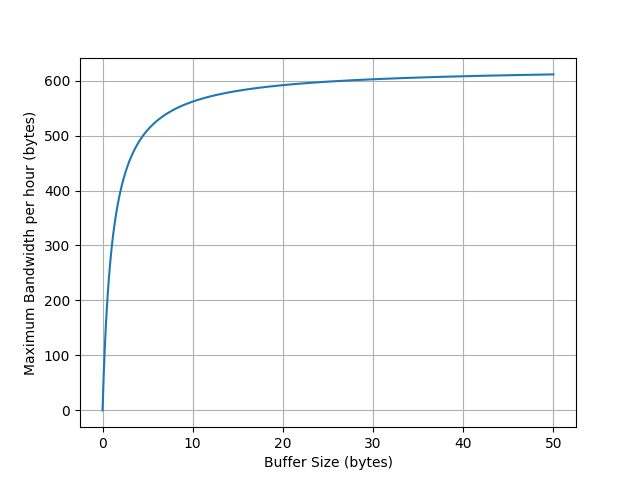
\includegraphics[scale=0.50]{images/trinket_plot.png}
    \caption{Maximum bandwidth per hour for a given buffer size (N)}
    \label{fig:buffer_plot}
\end{figure}

% DO NOT DELETE THESE COMMENTS @shivangi / @pranav
% from matplotlib.pyplot import *
% from numpy import *
% x=linspace(0,50,5000)
% y=5000*x/(8*x+9)
% plot(x,y)
% grid(True)
% xlabel("Buffer Size (bytes)")
% ylabel("Maximum Bandwidth per hour (bytes)")
% print(x)
% show()


Here buffer size is proportional to the number of comments on a given Github issue that is used to apply reactions on, thereby embedding the covert message. For example, a 32 bit buffer size will require 4 comments (8 reactions per comment, 32 / 8 = 4). Selecting an ideal buffer size is a crucial factor to maximize bandwidth of the covert channel while adhering to the API Rate limit. Consider the following two scenarios : 
\begin{itemize}
\item A low buffer size (or number of comments) will yield relatively less bandwidth per hour. This is because of the additional overhead involved in synchronizing the sender and receiver through repeated API calls to the header comment.
\item A very high buffer size would potentially use less overhead synchronization API calls, however it is relatively difficult to find an issue with higher number of comments.
\end{itemize}

\subsection{Experiments}

Analysing figure \ref{fig:buffer_plot}, it is evident that selecting a buffer size between 1-10 will yield less bandwidth. Hence, we experimented with buffer sizes ranging from 16 bytes to 32 bytes. 16 byte buffers were ideal for initial experimentation as it was easier to find issues with number of comments ranging from 16 to 32. For a given buffer size of N, at a minimum \(8N + 9\) API calls are needed to send the buffer. For example, for a buffer size of 16 bytes, 137 API calls are needed to transmit the buffer. During our experiments, we found that on an average, each transaction on the Github Reactions API takes around 0.14 seconds to complete. Thus, sending a 16 byte buffer over this covert channel will take at-least 137 * 0.14 = 19.18 seconds. This yields an average bandwidth of (16*8) / 19.18 = 6.67 bits / second.

In the real world however, diversity in messages can affect this calculated bandwidth quite drastically. Specifically, the frequency distribution of zeros in the binary representation of the data. This is due to the fact that encoding binary "zero" as a reaction doesn't require an API call as we're not setting a reaction for a zero bit. Thus, sending "11111111" is more costly than sending "10000000" over this covert channel. We conducted experiments with various 8 bit data and found the API response times to be as follows : 

\begin{table}[htbp]
\caption{API Response Times}
\begin{center}
\begin{tabular}{|c|c|}
\hline
\textbf{Binary} & \textbf{Time (secs)} \\
\hline
{00110000} & {0.695183} \\
\hline
{00110010} & {0.736954} \\
\hline
{00110111} & {1.12029} \\
\hline
{00110110} & {0.876527} \\
\hline
{01000100} & {0.602323} \\
\hline
\end{tabular}
\label{api_call_table}
\end{center}
\end{table}

Due to the repetitive pinging nature of the waitForSync function, the number of API calls required to send and receive the covert messages is not completely deterministic. Consider the following example : waitForSync is configured to ping the header comment every 2 seconds. Due to network lag, the receiver takes 8 seconds to complete reading the buffer and set the \emoji{thumbs-down} reaction on the header comment. At this point, the sender would have executed a total 4 API calls to check if \emoji{thumbs-down} has been set or not. 

\section{Limitations}

The Github API Rate Limit of 5000 requests per hour is the primary limiting factor of this covert channel. Due to this limitation, it is not advisable to deploy this covert channel as an infinitely listening service, similar to a background process or daemon. If deployed like this, the listener will consume 1800 API calls per hour just waiting for a connection (Assuming the sender doesn't send data for a given hour). Thus, the listener needs to be invoked explicitly when data needs to be ex-filtrated out of a system covertly. It is possible to increase the rate limit to 15,000 requests per hour through the Github Enterprise Cloud Account. This could be a potentially common scenario in a corporate environment, where companies tend to use Github's Enterprise offering, allowing an internal threat actor to use their Enterprise account to facilitate this higher rate limit. 

This covert channel can be considered quite noisy given the large number of API calls executed to covertly ex-filtrate data out. Even if the sender consumes most of the API rate limit, on an average the channel executes 1.38 API calls per second (adhering to the 5000 / hour rate limit). A well configured Intrusion Detection System (IDS) like snort or a corporate http proxy like Squid can track the unusually large number of specific API calls being made. This is covered more in the Detection section.

User attribution is another limitation of this covert channel. All reactions or Github API actions are tied to a specific user, which can be used to trace back a detected covert message back to the threat actor. Although it is possible for the receiver to perform unauthenticated API queries on public repositories, this is limited to 60 per hour and is limited to read-only transactions. Reactions cannot be made unauthenticated.

API Token Expiry is another limitation to consider. Although Github allows the creation of a token with unlimited expiration date, internal corporate policies usually forbid such practices. In a real world company using Github for SCM, an internal threat actor might be issued their employee access token with a limited expiry date. 

\section{Detection}

Snort is an Intrusion Detection System which does real time traffic analysis, packet sniffing and can work as a network intrusion detection system (NIDS). It has various network based sensors that monitors and filters the traffic \cite{b9}. The Snort HTTP decoder, HTTPInspect can be used to inspect unusual Github API calls. A Snort rule can be written to detect unusually large number of API calls to Github, and an alert can be triggered to a centralized dashboard. 

In a corporate setting, utilizing Github’s Enterprise offering, user access management to a company’s repositories is usually centrally managed. Although every user gets their own account, and thereby generates their own tokens, an administrator can view these token rate limits. Using this privilege, an automated alert can be generated to warn the administrator of unusually large API consumption. This could be a telltale sign of an active connection on this specific covert channel.


\section{Conclusion}
We were able to successfully create a covert channel using a pattern of emojis over a set of Github comments. Here the use of reactions are subjective in terms of how it will be translated into data. Also, reactions are not something instinctively observed \& conclusive for someone to realise it as a possible covert channel. These couple of factors strengthen the stealthiness of our channel. Moreover, from our experiments and analysis, we found that our covert channel yields a throughput of roughly 6 bits per second for an ideal buffer size of 16 bytes. We also demonstrated that messages with a lower frequency of 1s are transmitted faster in this covert channel. 

\section{Future Work}
As reactions can be applied to any comment on Github, there are two other potential channels to embed covert messages in. Github allows users to comment on commits and pull requests as well. These are additional avenues where covert messages can be embedded as reactions to comments. The covert channel code can be augmented in the future to implement the PullRequest and Commit APIs from the Github REST API to implement these channels. They can be used to multiplex multiple covert messages over a single connection. However, it must be noted that the Github API Rate limit is still applicable here. 

Github REST API has another rate limit for unauthenticated requests of 60 requests per hour. As this is limited to read-only queries, they could be potentially used for this channel's specific functionalities such as reading the header comment for synchronization. Github restricts these calls to 60 requests per hour per IP address, so this code can be threaded across multiple receiver IPs to increase the available bandwidth of the covert channel.

The current implementation does not transmit the message length over the covert channel. To accommodate this, the sender pads additional NULL terminators at the end of the message to fill up the buffer size. This requires redundant API calls on the receiver's end (8 times per redundant NULL terminator), which can be avoided if the message length is known to the receiver. This can be achieved by embedding the message length as an attribute during the start of the message.

The current implementation is hard-coded for 8 reactions in the Github API. Historically, Github has increased the number of reactions available. For example, till 2019 only 6 reactions where available on Github \cite{b8}, and it was increased to 8 recently. The code implementation can be augmented to make it agnostic to the number of reactions available, thus being able to automatically adjust the bandwidth based on available reaction pool.


\begin{thebibliography}{00}
\bibitem{b1}Ji, Liping, Yu Fan, and Chuan Ma. "Covert channel for local area network." 2010 IEEE International Conference on Wireless Communications, Networking and Information Security. IEEE, 2010. 
\bibitem{b2} Frikha, Lilia, and Zouheir Trabelsi. "A new covert channel in WIFI networks." 2008 Third International Conference on Risks and Security of Internet and Systems. IEEE, 2008.
\bibitem{b3} Qu, Haipeng, Purui Su, and Dengguo Feng. "A typical noisy covert channel in the IP protocol." 38th Annual 2004 International Carnahan Conference on Security Technology, 2004.. IEEE, 2004
\bibitem{b4} S. Dearstyne and D. Johnson, "Leveraging public posts and comments as covert channels," IWSSIP 2014 Proceedings, 2014, pp. 179-182.
\bibitem{b5} Egbert, Connor, Fawaz Alhenaki, and Daryl Johnson. "Leveraging a Music Streaming Platform in Establishing a Novel Storage Covert Channel." 2020 IEEE 45th Conference on Local Computer Networks (LCN). IEEE, 2020
\bibitem{b6} Ning, Jianxia, et al. "Secret message sharing using online social media." 2014 IEEE Conference on Communications and Network Security. IEEE, 2014.
\bibitem{b7}Chatziasimidis, Fragkiskos, and Ioannis Stamelos. "Data collection and analysis of GitHub repositories and users." 2015 6th International Conference on Information, Intelligence, Systems and Applications (IISA). IEEE, 2015.
\bibitem{b8}Borges, Hudson, Rodrigo Brito, and Marco Tulio Valente. "Beyond Textual Issues: Understanding the Usage and Impact of GitHub Reactions." Proceedings of the XXXIII Brazilian Symposium on Software Engineering. 2019.
\bibitem{b9} Chakrabarti, S., Mohuya Chakraborty, and Indraneel Mukhopadhyay. "Study of snort-based IDS." Proceedings of the International Conference and Workshop on Emerging Trends in Technology. 2010.
\end{thebibliography}

\end{document}
